\documentclass[12pt]{article}
\usepackage{a4wide}
\usepackage{amsmath,amssymb}
\usepackage{bm}
\usepackage[colorlinks]{hyperref}
\usepackage{graphicx}

\usepackage{algorithm}
\usepackage{algorithmic}

\usepackage{float}
\usepackage{bbold}
\usepackage{comment}
\usepackage{mathtools}

%\usepackage{caption,refstyle}




\usepackage[french]{babel}
\usepackage[T1]{fontenc}
\usepackage{lmodern}

\DeclareUnicodeCharacter{2009}{\,} 
\usepackage[standard]{ntheorem}


\begin{document}

\begin{titlepage}
\title{Algorithme Glouton faible par apprentissage}
\author{Congo Job
\\ Stage Master 1 de juin à juillet 2022 sous la direction de Joubine Aghili \\
 IRMA, Université de Strasbourg, France}
\date{ 22 août 2022}

\begin{figure}[b!]
\centering
\vfill

\includegraphics[scale=0.16]{logo-unistra.pdf}
\hspace{0.5 cm}

\includegraphics[scale=0.16]{logo_irma.pdf}
\hspace{0.5 cm}

\includegraphics[scale=0.16]{logoCSMI.pdf}
\end{figure}
\end{titlepage}


\maketitle
\thispagestyle{empty}


\newpage

\tableofcontents

\newpage

\section{Introduction}

\subsection{Contexte du stage}

%---- presenter IRMA,...
Ce stage est réalisé à Institut de Recherche de Mathématiques Avancées (IRMA). L’IRMA, créé en 1966, est depuis 1997 une unité mixte de recherche
sous la double tutelle du CNRS et de l’Université de Strasbourg. Il fait partie de l’UFR de Mathématique et Informatique.
Elle compte quelques 130 membres, dont 87 chercheurs et enseignants-chercheurs permanents et une quarantaine de non-permanents répartis en 7 équipes de recherche. 
C'est avec l'équipe "Modélisation et contrôle" que le stage a eu lieu. 
Cette équipe s'intéresse à l’analyse des EDP, à l'optimisation, à la théorie du 
contrôle, au calcul scientifique et haute performance, et à la statistique. Ce stage a eu lieu du 1 juin 2022 au 31 juillet 2022. On retrouvera tous les documents du stage dans ce lien : \url{https://github.com/master-csmi/2022-stage-job-br}.





\subsection{Objectif du stage}

%---- motiver le sujet et objectif stage

Dans le contexte de la résolution numérique d'une EDP paramétrée, la méthode des bases réduites \cite{Gianluigi Rozza} s'avère souvent être une option de premier choix.
Elle repose sur l'hypothèse que l'ensemble des solutions du problème de l'EDP est *proche*, en un certain sens, d'un espace affine de petite dimension.
Dès lors, une stratégie en deux temps permet d'évaluer la solution $u(\mu)$ pour un paramètre $\mu$ donné, en un temps de calcul bref.
La dite stratégie se decompose en une phase hors-ligne (*offline*) où tous les précalculs sont effectués une fois pour toutes, et une phase en-line (*online*) où les évaluations nécessitant un temps de calcul courts y sont faits.
Lors de la phase hors-ligne, un temps important est consacré à la construction d'une petite famille de solutions indexée par des paramètres du problème, appelée *base réduite*.
Cette famille est construite grâce à un algorithme dit glouton qui à chaque étape maximise une erreur de projection pour trouver un paramètre $\mu^*$ optimal.
L'erreur de projection étant inaccessible en pratique, on utilise plutôt des bornes sur celle-ci.
L'objectif de ce stage est de construire un modèle par réseaux neuronaux pouvant se substituer à cette erreur et enfin comparer l'efficacité de l'algorithme Glouton avec celui-ci. Une première étape consiste à implémenter un exemple en 1d en Python avec la méthode des éléments finis et donner une validation, puis implémenter la méthode des bases réduites et donner une validation, enfin entrainer un réseau de neurone apprenant l'erreur de projection à l'aide de PyTorch/TensorFlow. Par la suite effectuer la même chose sur un exemple 2D.






%---- détail objectif stage
Pour ce faire, on commencera par s'intéresser à une EDP en 1D de type réaction-diffusion s'écrivant : 

$$
\begin{cases} 
- \frac{\partial }{\partial x}(D \cdot \frac{\partial u}{\partial x}) + u = f  & \Omega   \\
u = 0  & \partial \Omega \\
D(x) = 
\begin{cases} 
1 , x \in \Omega _{1} \\
\mu , x \in \Omega _{2}
\end{cases} \\
\text{Avec } \Omega =  ]0,1[ \text{   } \Omega _{1} = \Omega \backslash\ \Omega_{2}  \\
\Omega _{2} = ]0.19, 0.21[ \cup  ]0.39, 0.41[ \cup ]0.59, 0.61[ 
\cup ]0.79; 0.81[ 
\label{moneq}
\end{cases}%
(\ref{moneq})
$$


On résoudra le problème 1D \eqref{moneq} par la méthode des éléments finis et en même temps on construira un solveur $u_{EF}(\mu)$. Cette fonction $u_{EF}(\mu)$ renverra pour un $\mu$ donné la solution élément fini associé. Puis nous mettrons en œuvre la méthode des bases réduites à l'aide de cette fonction $u_{EF}(\mu)$ et de l'algorithme Glouton fort. L'algorithme Glouton fort utilise les solutions ainsi obtenues par $u_{EF}(\mu)$ pour engendrer un espace vectoriel de dimension réduite $V_{N_0} = Vect(u_1,u_2,..., u_{N_0})$. Le travail principal de cet algorithme consiste à maximiser l'erreur de projection $\Delta(V_{N_0}, \mu) =||u_{EF}(\mu) - P_{V_{N_0}}u_{BR}(\mu)||$. Enfin, nous entraînerons par réseau de neurone un modèle $\Delta^{NN}(\mu)$ qui remplacera $\Delta(V_{N_0}, \mu)$ dans l'algorithme Greedy Fort. Nous espérons alors, grâce à ce modèle, évaluer rapidement l'erreur pour tout point $\mu$, et de profiter de son caractère différentiable pour obtenir une base réduite de meilleure qualité après optimisation.


\subsection{Etat de l'art}
\subsection{Plan du rapport }

Dans la section \ref{ef}, nous resolvons le problème élément finis et ferons une etude de convergence, dans la section \ref{br} la résolution du modèle réduit avec l'algorithme Glouton fort.









\section{Elements finis}
\label{ef}

On s'intéresse au problème 1D suivant de \cite{Alexandre Ern} :

\begin{equation}\label{moneq2}
\begin{cases} 
- \frac{\partial }{\partial x}(D \cdot \frac{\partial u}{\partial x}) + u = f , & \Omega   \\
u = 0 , & \partial \Omega \\
D(x) = 
\begin{cases} 
1 , x \in \Omega _{1} \\
\mu , x \in \Omega _{2}
\end{cases}
\end{cases}
\end{equation}

\subsection{Formulation Variationnelle}

On multiplie \eqref{moneq2} par $v \in H_{0}^{1}(\Omega)$ et integre sur $\Omega$ :

\begin{equation} \label{eq:1}
\int_{\Omega} -v(D.u')' + \int_{\Omega} vu = \int_{\Omega} fv 
\end{equation}

Après intégration par partie où on a utilisé $ v_{|\partial \Omega} = 0 $, on a :
$$
 \int_{\Omega} D.v'u' + \int_{\Omega} vu = \int_{\Omega} fv 
$$

On pose :
$$
\forall u, v \in H_{0}^{1}(\Omega) 
\hspace{0.5 cm}
a(u,v;\mu) := \int_{\Omega} \mathbb{1}_{\Omega_{1}}v'u' + \mu\int_{\Omega} \mathbb{1}_{\Omega_{2}} v'u' + \int_{\Omega} vu 
\text{, }
\hspace{0.5 cm}
l(v) := \int_{\Omega} fv.
$$

Et la formulation variationnelle de \eqref{eq:1} se réécrit, trouver 
$u \in H_{0}^{1}(\Omega)$ tel que :


\begin{equation} \label{eq:2}
a(u,v;\mu) = l(v) , \forall v \in H_{0}^{1}(\Omega)
\end{equation}



%------- dire éventuellement que le pb est bien posé







% \subsection{Théorème de Lax-Milgram }




\subsection{Discrétisation du problème }

On va décrire le problème éléments finis pour le problème 
 \eqref{eq:2} avec une approximation $\mathbb{P}^{1}$, pour plus d'informations voir [Grégoire Allaire, Analyse num et optimisation]


\subsubsection{Construction des espaces d’approximation } 

Soit $\Omega $ un segment, que l'on décompose en $\Omega_{1}$ et 
$\Omega_{2}$ disjoints et construit un maillage équidistant : $$ \Omega = 
\bigcup_{i =0} ^{Nel - 1} K_i $$ 
tel que :
\begin{enumerate}
 \item $\Omega_2 = ]0.19,0.21[\cup]0.39,0.41[\cup]0.59,0.61[\cup]0.79,0.81[\text{ et } \Omega_{1} = \Omega \backslash\ \Omega_{2}$.
 \item $Nel$ est le nombre d'éléments du maillage et $h$ le pas constant vaut $ \frac{1}{Nel - 1}$.
 \item $ K_i \text{ la maille } [x_i, x_{i+1}] \text{ avec } x_i = ih \text{, } \forall i \in \{0,..., Nel-1 \}$.
 \item On suppose que chaque maille $K_i$ se trouve soit dans $\overline{\Omega_1}$ soit dans $\overline{\Omega_2}$.
\end{enumerate}

 
%---- mettre élément finis  ???
\begin{comment}
Après la décomposition de $\Omega$, nous définissons l’élément fini $(K_i,P_{K_{i}},\Sigma_{K_{i}})$ avec $\Sigma_{K_{i}} = \{ x_{i-1},x_{i} \}  \text{ et }  P_{K_{i}} = P^{1}(K_{i})$ et les fonctions de base sont alors:
$$ p_{x_{i}} = \frac{x- x_{i+1}}{x_{i} - x_{i+1}}  \text{ et } p_{x_{i+1}} = \frac{x- x_{i}}{x_{i+1} - x_{i}}$$

 \noindent Puis, nous construisons l’espace d’approximation $V_h$ des fonctions $\varphi_{i} : \Omega \longrightarrow \mathbb{R}$ de la manière 
suivante :
\end{comment}


Après la décomposition de $\Omega$, nous construisons l’espace d’approximation $V_h$ des fonctions $\varphi_{i} : \Omega \longrightarrow \mathbb{R}$ de la manière suivante :

 \noindent Après la décomposition de $\Omega$, nous construisons l’espace d’approximation $V_h$ des fonctions $\varphi_{i} : \Omega \longrightarrow \mathbb{R}$ de la manière 
suivante :

$$
\forall i \in [0,Nel-1], 
\varphi_{i} (x) = 
\begin{cases}
\frac{x-x_{i-1}}{h}, x \in [x_{i-1}, x_{i}]\\
-\frac{x-x_{i+1}}{h}, x \in [x_{i}, x_{i+1}] \\
0 \text{, sinon}
\end{cases}
$$



%---- mettre image fonction de base phi_i,phi_i-1,phi_i+1


\begin{figure}[H]
\begin{center}
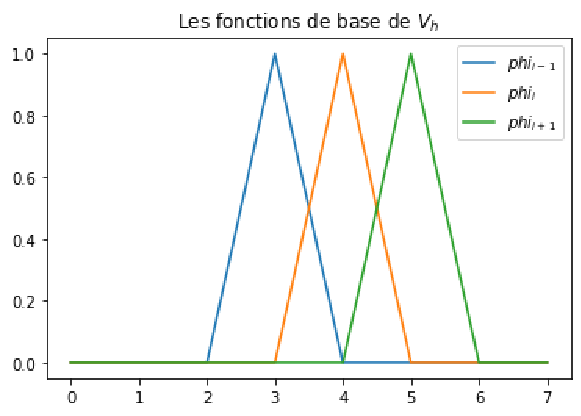
\includegraphics[scale=1]{fct_baseVh.pdf}
\caption[]{Illustration des fonctions de base}
\end{center}
\end{figure}


\noindent Et sa dérivée est définie, lorsque c'est possible, par la formule :

$$
\forall i \in [0,Nel-1], 
\varphi_{i}'(x) = 
\begin{cases}
\frac{1}{h}, x \in]x_{i-1}, x_{i}[\\
-\frac{1}{h}, x \in]x_{i}, x_{i+1}[\\
0 \text{, sinon} 
\end{cases}
$$


\noindent L'espace d'approximation $\mathbb{P}^1$ est alors : $$ V_{h} = Vect (\{\varphi_{i}\})$$

\noindent Comme $ V_{h}$ est l’espace d’approximation $\mathbb{P}^1$ alors une discrétisation possible de $H^{1}_{0}(\Omega)$ est l’espace $V_{h,0}$ défini par : 
$$ 
V_{h,0} = \{u \in V_{h} | \text{ } \forall i \in \{0,..., Nel-1 \} \text{ } u_{|K_{i}} \in \mathbb{P}^1(\Omega) \text{ et } u_{| \partial \Omega} = 0 \} 
$$



\subsubsection {Construction des matrices éléments finis}

\noindent En remplacant $H_{0}^{1}(\Omega)$ par $V_{h,0}$, on va chercher à résoudre le problème approché : 

\begin{equation} \label{eq:3}
\text{Trouver } u_h \in V_{h,0} \text{ tel que : } a(u_h, v_h;\mu) = l(v_h), \forall v_h \in V_{h,0}
\end{equation}

\noindent On sait que $\forall u_h \in V_{h,0}$, $u_h = \sum_{i = 0}^{Nel-1} \alpha_i\varphi_{i}$ donc \eqref{eq:3} devient

\begin{equation*} 
 \sum_{i = 0}^{Nel-1}\alpha_ia(\varphi_{i}, v_h;\mu) = l(v_h), \forall v_h \in V_{h,0}
\end{equation*}

\noindent En prenant $v_h = \varphi_{j}$ on a :
\begin{equation*} 
 \sum_{i = 0}^{Nel-1}\alpha_i a(\varphi_{i}, \varphi_{j};\mu) = l(\varphi_{j}), \forall \varphi_{j} \in V_{h,0}
\end{equation*}

\noindent Notons 
$$
A_{\mu} := \begin{pmatrix}
 &  &  & & \\
 &  &  &  & \\
 &  &  a(\varphi_{i},\varphi_{j};\mu)  &  & \\
  &  &  & & \\
 &  &  & &
\end{pmatrix} 
X :=\begin{pmatrix}
 \alpha_0   \\
 .  \\
 . \\
 . \\
\alpha_{Nel-1} 
\end{pmatrix} \text{ et } b := \begin{pmatrix}
\\
\\
l(\varphi_{j}) \\
\\

\\
\end{pmatrix}
$$

\noindent Résoudre \eqref{eq:3} revient à touver $X$ tel que $$ A_{\mu}X=b$$
où :
\begin{enumerate}
    \item $A_{\mu} = A_{1} + \mu A_{2} + M $  
    \item $A_{1} = \int_{\Omega} \mathbb{1}_{\Omega_{1}} \varphi'_{i} \varphi'_{j}    \text{ ,  } A_{2} = \int_{\Omega} \mathbb{1}_{\Omega_{2}} \varphi'_{i} \varphi'_{j} \text{  ,  }  M = \int_{\Omega} \varphi_{i} \varphi_{j}$
    \item  $ b = \int_{\Omega} f \varphi_{j}$
\end{enumerate}

\noindent Après calculs on a :

$$
(A_{1})_{ij} = 
\begin{cases}
a(\varphi_{i}, \varphi_{j}) = 0, x \notin [x_{i-1}, x_{i+1}] \\
a(\varphi_{i}, \varphi_{i+1}) = -\frac{1}{h}, x \in [x_{i}, x_{i+1}] \\
a(\varphi_{i}, \varphi_{i-1}) = -\frac{1}{h}, x \in [x_{i-1}, x_{i}] \\
a(\varphi_{i}, \varphi_{i}) = \frac{2}{h}, x \in [x_{i-1}, x_{i+1}] 
\end{cases}
$$

\noindent De même pour $ A_{2} $ on a :

$$
(A_{2})_{ij} = 
\begin{cases}
a(\varphi_{i}, \varphi_{j}) = 0, x \notin [x_{i-1}, x_{i+1}] \\
a(\varphi_{i}, \varphi_{i+1}) = -\frac{1}{h}, x \in [x_{i}, x_{i+1}] \\
a(\varphi_{i}, \varphi_{i-1}) = -\frac{1}{h}, x \in [x_{i-1}, x_{i}] \\
a(\varphi_{i}, \varphi_{i}) = \frac{2}{h}, x \in [x_{i-1}, x_{i+1}] 
\end{cases}
$$

\noindent Pour la matrice de masse M on a :
$$
(M)_{ij} = 
\begin{cases}
a(\varphi_{i}, \varphi_{j}) = 0, x \notin [x_{i-1}, x_{i+1}] \\
a(\varphi_{i}, \varphi_{i+1}) = \frac{h}{6}, x \in [x_{i}, x_{i+1}]\\
a(\varphi_{i}, \varphi_{i-1}) = \frac{h}{6}, x \in [x_{i-1}, x_{i}] \\
a(\varphi_{i}, \varphi_{i}) = \frac{2h}{3}, x \in [x_{i-1}, x_{i+1}] 
\end{cases}
$$


\noindent Pour calculer le second membre, nous utilisons la méthode des trapèzes par morceaux.

$$
b = \int_{\Omega} f \varphi_j = \sum_{j = 0}^{Nel -1} \int_{x_{j}}^{x_{j+1}} f \varphi_{j}. 
$$

\noindent En supposant que $ f = 1 $, on a :
$$
b_{j} = \int_{x_{j-1}}^{x_{j+1}} f \varphi_j 
= \frac{(h_{j} + h_{j+1})}{2}, x \in [x_{j-
1}, x_{j+1}]. 
$$

\noindent En fin, on obtient :

$$
b_{j} = h, \forall j \in \{0,..., Nel-1\}
$$
 
%----- parler des conditions au limites
Pour respecter les conditions aux bords, nous avons rendu les lignes associées aux degrés de liberté de Dirichlet, nulles, sauf sur la diagonale de $A_{\mu}$ la valeur 1. Pour finir les matrices se réécrivent :
$$
b_{j} =
\begin{cases}
h, \forall j \in \{1,..., Nel-2\} \\
0 \text{, sinon} 
\end{cases}
(A_{\mu})_{ij} =
\begin{cases}
A_{ij}, \forall i, j \in \{1,..., Nel-2\} \\
1 \text{, lorsque } $(i, j) = (0,0)$ \text{  ou  } $(i, j) = (Nel-1,Nel-1)$ \\
0 \text{, sinon} 
\end{cases}
$$
Pour $\mu = 1 $ et $Nel = 10 $, on a :

\begin{center}
$
A_1 = \begin{pmatrix}
1 & 0 & 0 & 0 & 0 & 0 & 0 & 0 & 0 & 0  \\
-9 & 18 & -9 & 0 & 0 & 0 & 0 & 0 & 0 & 0  \\
0 & -9 & 18 & -9 & 0 & 0 & 0 & 0 & 0 & 0  \\
0 & 0 & -9 & 18 & -9 & 0 & 0 & 0 & 0 & 0  \\
0 & 0 & 0 & -9 & 18 & -9 & 0 & 0 & 0 & 0  \\
0 & 0 & 0 & 0 & -9 & 18 & -9 & 0 & 0 & 0  \\
0 & 0 & 0 & 0 & 0 & -9 & 18 & -9 & 0 & 0  \\
0 & 0 & 0 & 0 & 0 & 0 & -9 & 18 & -9 & 0  \\
0 & 0 & 0 & 0 & 0 & 0 & 0 & 0 & 0 & 1  \\
\end{pmatrix}
$
\end{center}

\begin{center}

$
A_2 = \begin{pmatrix}
0 & 0 & 0 & 0 & 0 & 0 & 0 & 0 & 0 & 0  \\
0 & 0 & 0 & 0 & 0 & 0 & 0 & 0 & 0 & 0  \\
0 & 0 & 9 & 0 & 0 & 0 & 0 & 0 & 0 & 0  \\
0 & 0 & 0 & 0 & 0 & 0 & 0 & 0 & 0 & 0  \\
0 & 0 & 0 & 0 & 9 & 0 & 0 & 0 & 0 & 0  \\
0 & 0 & 0 & 0 & 0 & 9 & 0 & 0 & 0 & 0  \\
0 & 0 & 0 & 0 & 0 & 0 & 0 & 0 & 0 & 0  \\
0 & 0 & 0 & 0 & 0 & 0 & 0 & 9 & 0 & 0  \\
0 & 0 & 0 & 0 & 0 & 0 & 0 & 0 & 0 & 0  \\
0 & 0 & 0 & 0 & 0 & 0 & 0 & 0 & 0 & 0  \\
\end{pmatrix}
$
\text{et }
$
b = \begin{pmatrix}
0 \\
0.11 \\
0.11 \\
0.11 \\
0.11 \\
0.11 \\
0.11 \\
0.11 \\
0.11 \\
0 \\
\end{pmatrix}
$
\end{center}

\begin{center}
$
M = \begin{pmatrix}
0 & 0 & 0 & 0 & 0 & 0 & 0 & 0 & 0 & 0  \\
0.019 & 0.074 & 0.019 & 0 & 0 & 0 & 0 & 0 & 0 & 0  \\
0 & 0.019 & 0.074 & 0.019  & 0 & 0 & 0 & 0 & 0 & 0  \\
0 & 0 & 0.019 & 0.074 & 0.019  & 0 & 0 & 0 & 0 & 0  \\
0 & 0 & 0 & 0.019 & 0.074 & 0.019  & 0 & 0 & 0 & 0  \\
0 & 0 & 0 & 0 & 0.019 & 0.074 & 0.019  & 0 & 0 & 0  \\
0 & 0 & 0 & 0 & 0 & 0.019 & 0.074 & 0.019  & 0 & 0  \\
0 & 0 & 0 & 0 & 0 & 0 & 0.019 & 0.074 & 0.019  & 0  \\
0 & 0 & 0 & 0 & 0 & 0 & 0 & 0.019 & 0.074 & 0.019   \\
0 & 0 & 0 & 0 & 0 & 0 & 0 & 0 & 0 & 0  \\
\end{pmatrix} 
$
\end{center}














\subsection{Validation}
On vérifie que si $\mu = 1 $ la solution éléments finis $u_{EF}$ est cohérente avec la solution exacte $u_{ex}$. En effet, si $\mu = 1 $, alors $D(x) \equiv 1 $ et le système d'équations \eqref{moneq2} devient :

\begin{equation}\label{eqnum1}
\begin{cases}
-u'' + u = 1 \\
u|_{\partial \Omega} = 0
\end{cases}
\end{equation}



Ce nouveau problème \eqref{eqnum1} admet une unique solution $u_{ex}(x)$ :
$$
\forall x \in \Omega, u_{ex}(x) = C_{1}\exp(-x) + C_{2}\exp(x) +1 \text{, avec } C_{1} = \frac{1-e}{e - e^{-1}} \text{ et } C_{2} = \frac{e^{-1} - 1}{e - e^{-1}} $$

%---- presenter les résultats en norme L2et H1
Pour vérifier la convergence de $u_{EF}$ la solution approchée du problème $\eqref{eqnum1}$ vers la solution exacte $u_{ex}$, nous avons les résultats ci-dessous qui permettent d’estimer l’erreur $u_{ex} - u_{EF}$ en norme $L^{2}(\Omega)$ et $H^{1}(\Omega)$. On notera $||.||_1$ la norme $H^{1}$, et $||.||_0$ la norme $L^{2}$. On rappelle les estimations d'erreurs que l'on retrouve dans \cite{Bopeng RAO} à la page 57.

\begin{Proposition}
On suppose que la solution du problème $u$ est dans $H^{2}(\Omega)$
et on note $u_{h}$la solution du problème approché $\eqref{eqnum1}$ 
 Alors il existe une constante $c$ dépendante seulement de $\Omega$ telle que
 $$
 ||u-u_{h}||_{1,\Omega} \leq ch|u|_{2,\Omega}.
 $$
\end{Proposition}

\begin{Proposition}
On note $u$ la solution du problème et $u_{h}$ la solution du problème approché $\eqref{eqnum1}$ Alors il existe une constante $c$ dépendante seulement de $\Omega$ telle que
 $$
 ||u-u_{h}||_{0,\Omega} \leq ch^{2}|u|_{2,\Omega}.
 $$
\end{Proposition}


%------- à revoir


\noindent Pour tout $u \in V_{h,0}$, on a :
$$
|| u||_{L^{2}(\Omega)}^{2} = \int_{\Omega} u^2 dx = \sum_{i, j = 1}^{N} u_i u_j\int_{\Omega} \varphi_i\varphi_j dx 
$$

$$
|| u||_{H^{1}(\Omega)}^{2} = \int_{\Omega} u^2 + (u')^2 dx \\
= \sum_{i, j = 1}^{N} u_i u_j\int_{\Omega} \varphi_i\varphi_j dx + 
\sum_{i, j = 1}^{N} u_i u_j\int_{\Omega} \varphi_i'\varphi_j'dx \\
$$
\noindent En posant : 
$$ 
U :=\begin{pmatrix}
u_{0}\\

. \\

. \\

. \\
u_{Nel-1}\\
\end{pmatrix}
N := A_1 + A_2
$$

\noindent Finalement on en déduit :
$$
||u||_{L^{2}(\Omega)}^{2} = U^{T}MU \text{       et        } ||u||_{H^{1}(\Omega)}^{2} = U^{T}(M+N)U 
$$


\begin{figure}[H]
\begin{center}
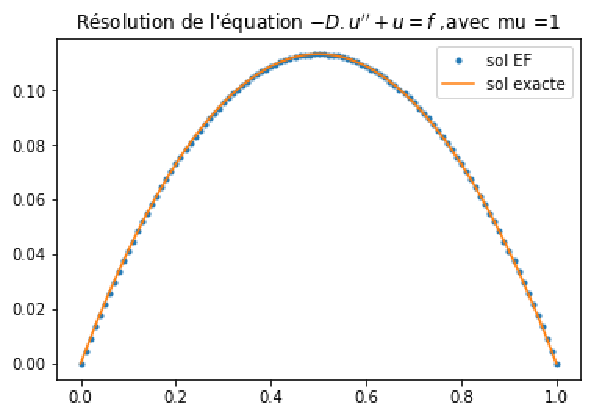
\includegraphics[scale=1]{sol_ef_exa.pdf}
\caption[]{Solution exacte  $u_{ex}$ et Solution élément fini $u_{EF}$  }
\end{center}
\end{figure}


\begin{figure}[H]
\begin{center}
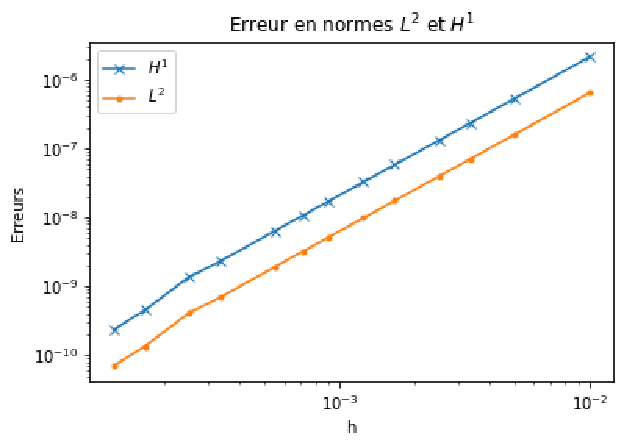
\includegraphics[scale=1]{erreurL2H1V2.pdf}
\caption[]{Erreurs $|| u_{ex} - u_{EF}||_{L^{2}}$ et $|| u_{ex} - u_{EF}||_{H^{1}}$ en fonction de h}
\end{center}
\end{figure}


Pour différentes valeurs de Nel le nombre d'éléments du maillage dans \\
\{100,200,300,400,600,800,1100,1400,1800,3000,4000,6000,8000,10000\}, nous avons résolu le problème \eqref{eqnum1} et calculé l'erreur entre $u_{ex}$ et $u_{EF}$ en norme $H^1$ et $L^{2}$. La pente de l'erreur est de $2$ en norme $H^1$ et $L^{2}$.


\begin{comment}
    , ce qui est conforme aux attentes théoriques
\end{comment}






\section{Modèle réduit}
\label{br}


\subsection { Formulation du problème réduit }

\noindent La méthode des bases réduites s'appuie sur le fait que les solutions de l'EDP vivent sur une variété de faible dimension, approchable par un espace affine lui aussi de petite dimension. Dans notre cas, la variété est définie par :

$$ V =  \{ u(\mu) \in H^{1}_{0}(\Omega) | \mu \in P_{test} \} \text{ avec } P_{test} \subset \mathbb{R^{+*}}$$

\noindent De la même manière que nous approchons l’espace $H^{1}_{0}(\Omega)$ par l’espace discret $V_{h}$, nous construisons une approximation $V_{N_{0}}$ de $V$ de la manière suivante :

$$ V_{N_{0}} =  \{ u(\mu) \in  V | \mu \in P_{trial} \} \text{ avec } P_{trial} \subset \mathbb{R^{+*}}$$

\noindent La méthode des bases réduites repose sur une projection de type Galerkin sur un espace $V_{N_{0}}$ de dimension $N_{0}$, avec  $N_0\ll N $ et $N = \text{dim($V_{h}$)}$. Nous verrons comment construire l’espace $V_{N_{0}}$ afin qu’il approche au mieux $V_{h}$.

\noindent En remplaçant $V_{h}$ par $V_{N_{0}}$ dans le problème approché \eqref{eq:3}, le problème réduit s'écrit :
\begin{equation}
\label{eq:4}
 \text{ Trouver } u^{BR}_{\mu} \in V_{N_{0}} \text{ tel que } a_{\mu}(u^{BR}_{\mu},u_i) = b(u_i) , \forall i \in \{1,...,N_0\}   
\end{equation}



\subsection { Espace des bases réduites $V_{N_{0}}$ }

\noindent Pour commencer, introduisons l'ensemble de paramètres $P_{test}:= \{\mu_1,..., \mu_{M} \}$. Ce essemble, de cardinal M, a des valeurs strictement positives. Ensuite nous deffinissons l'ensemble $P_{trial}$ de dimension $N_{0}$ : 
$$P_{trial} := \{\mu_1,..., \mu_{N_0} \} \text{ avec } N_0\ll M$$ à laquel on associe l’espace des bases réduites 
$$ V_{N_{0}} := vect(u_1,u_2,..., u_{N_0}) $$

\noindent Les fonctions $u_i$ pour $ i \in P_{trial}$ sont appelés « snapshot ». Elles sont obtenues en résolvant le problème approché par éléments finis. La construction de l'espace réduit $V_{N_{0}}$, qui approche au mieux $V_{h}$, est faite à l’aide de l’algorithme glouton dont une implémentation est donnée ci-dessous.



\begin{algorithm}
\caption{Algorithme Glouton}
\begin{algorithmic}
\REQUIRE $P_{test}$ ensemble , $u_{EF}(\mu)$ et $u_{BR}(\mu)$ 2 fonctions
\STATE {choisir $\mu_1 $ de manière aléatoire}
\STATE {$u_1 = u_{EF}(\mu)$}
\STATE {$B_1 = Vect(u_1)$}
\FOR {$i$ allant de 2 à ${N_0}$ }
\STATE {$u_i := \underset{\mu \in P_{test}}{argmax }(||u_{EF}(\mu) - P_{B_i}u_{BR}(\mu)||)$}
\STATE {$B_i := Vect(u_1,...,u_i)$}
\ENDFOR
\ENSURE retourner $B_{N_0}$ \\
\end{algorithmic}
\end{algorithm}







\subsection{ Matrices réduites}

\noindent On sait que $u^{BR}_{\mu}$ et $u_i$  se décomposerntsous la forme 
$$ 
u_{BR}^{\mu} = \sum_{i = 1}^{N_0} X^{BR}_{\mu, i}u_i 
\text{ et } 
u_i = \beta_0 \varphi_0 + ... + \beta_{Nel-1} \varphi_{Nel-1} 
$$

Et par billinéaire et linéarité de $l$ et $a_{\mu}$, on a :
$$
a_{\mu}(u^{BR}_{\mu}, u_i) = \sum_{i= 1}^{N_0}
\sum_{k, j= 0}^{Nel-1} X^{BR}_{\mu, i} 
\beta_{i, k} \beta_{i, j} a_\mu(\varphi_{k}, \varphi_{j})
$$
$$
l(u_i) = \sum_{i= 1}^{N_0}\sum_{j= 0}^{Nel-1} \beta_{i, j} l(\varphi_{j})
$$

\noindent Posons maintenant
$$
X^{BR} = \begin{pmatrix}
X^{BR}_{\mu,1} \\

. \\

. \\

. \\
X^{BR}_{\mu,N_0} \\
\end{pmatrix} 
U = \begin{pmatrix}
u_1, ..., u_{N_0}
\end{pmatrix} 
$$

\noindent On réécrit l'équation \eqref{eq:4} sous forme matricielle :
$$
(U^{T}A_{\mu}U)X^{BR} = 
U^{T}(A_0 + M)U + \mu U^{T}A_1U = U^{T}b \\
$$
Notons 
$$
V_{0}^{BR} := U^{T}(A_0 + M)U \text{   et   }  V_{1}^{BR} := U^{T}A_1U
$$
Ainsi on a les relations suivantes :
$$
B^{BR} := U^{T}b \text{    et    } A^{BR}_{\mu} = V_{0}^{BR} + \mu V_{1}^{BR}
$$

\noindent Résoudre le problème réduit \eqref{eq:4} revient finalement à trouver $X^{BR}$ tel que :
$$A^{BR}_{\mu} X^{BR} = B^{BR} $$ 


\noindent La méthode des bases réduites se décompose en deux étapes : <<hors-ligne>> et <<en-ligne>>. À l’étape hors-ligne, le vecteur $B^{BR}$ et les matrices $V_{0}^{BR}$ et $V_{1}^{BR}$ sont calculées une seule fois. À l’étape en-ligne, pour un certain $\mu \in P_{M}$, on assemble la matrice $A^{BR}_{\mu}$ et resout le système réduit $$A^{BR}_{\mu} X^{BR} = B^{BR}$$









\subsection{Etude du modèle réduit}
Dans cette section, nous allons analyser la solution réduite du problème \eqref{eqnum1}. Pour ce faire, il faut d'abord choisir la valeur $N_{0}$ afin d'appliquer l'algorithme glouton.

Après la construction de $V_{0}^{BR}$ et $V_{1}^{BR}$ pour diverses valeurs de $N_{0}$, nous avons calculé leur conditionnement respectif. Quand $N_{0}$ est supérieur ou égale à 5, le problème devient mal conditionné et leurs conditionnements sont alors de l'ordre de $10^{16}$ d'après le graphique \eqref{fig:1}. Lorsque $N_{0}$ est égal à 2, le résultat est très insuffisant. Les valeurs convenables de $N_{0}$ sont donc 3,4,5. 
Dans la suite, nous fixons $N_{0}$ à 3 pour avoir un conditionnement peu élevé.


\begin{figure}[H] 
\begin{center}
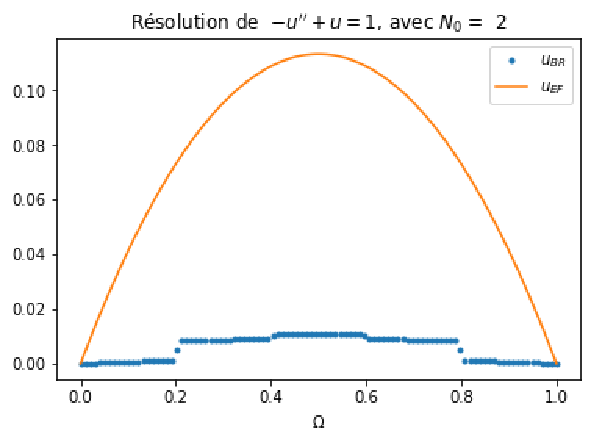
\includegraphics[scale=1]{sol_br_ef_2.pdf}
\caption[]{Solutions Eléments Finis et Base Réduite  }
\end{center}
\label{fig:1}
\end{figure}

\begin{figure}[H] 
\begin{center}
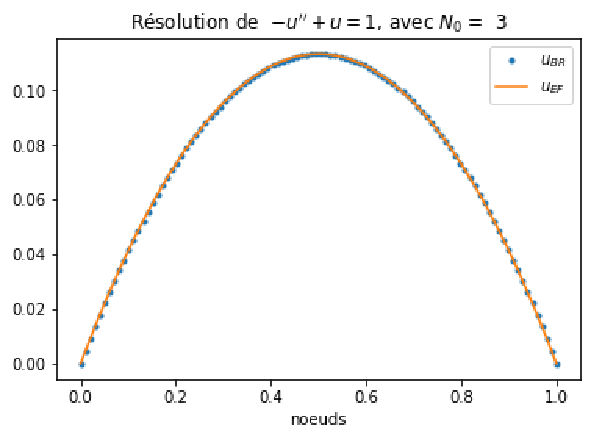
\includegraphics[scale=1]{sol_br_ef_3.pdf}
\caption[]{Solutions Eléments Finis et Base Réduite  }
\end{center}
\label{fig:1}
\end{figure}

\begin{figure}[H] 
\begin{center}
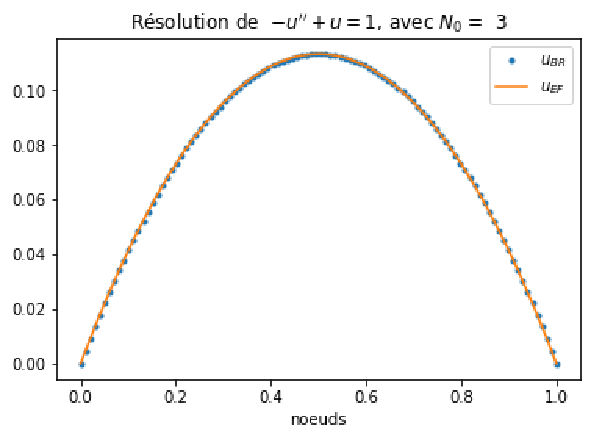
\includegraphics[scale=1]{sol_br_ef_3.pdf}
\caption[]{Solutions Eléments Finis et Base Réduite  }
\end{center}
\label{fig:1}
\end{figure}

\begin{figure}[H] 
\begin{center}
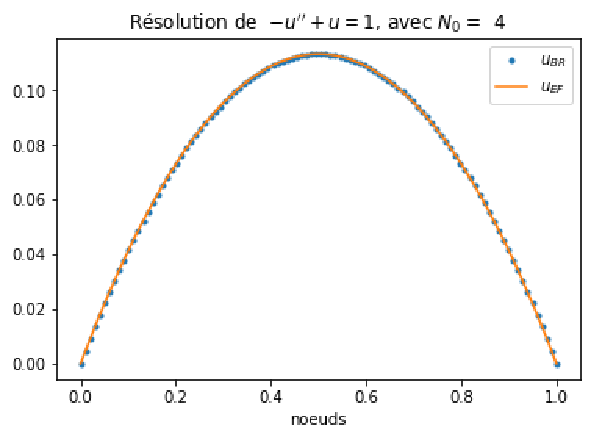
\includegraphics[scale=1]{sol_br_ef_4.pdf}
\caption[]{Solutions Eléments Finis et Base Réduite  }
\end{center}
\label{fig:1}
\end{figure}

\begin{figure}[H] 
\begin{center}
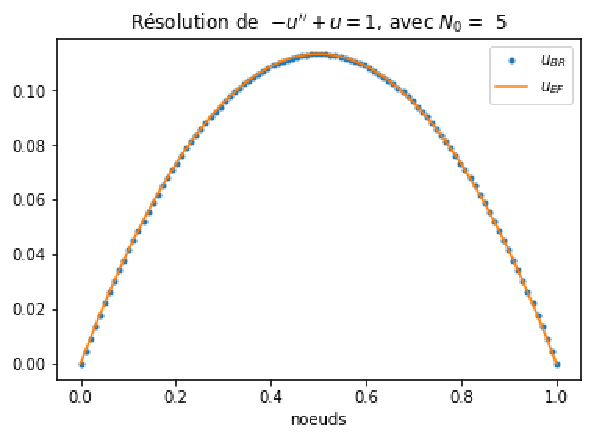
\includegraphics[scale=1]{sol_br_ef_5.pdf}
\caption[]{Solutions Eléments Finis et Base Réduite  }
\end{center}
\label{fig:1}
\end{figure}



\begin{figure}[H] 
\begin{center}
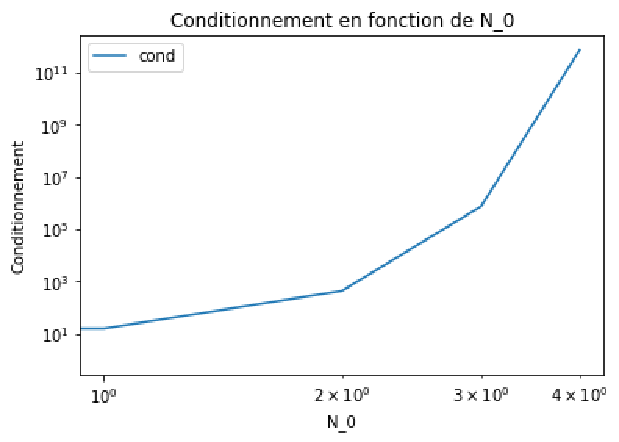
\includegraphics[scale=1]{cond.pdf}
\caption[]{Evolution du conditionnement }
\end{center}
\label{fig:1}
\end{figure}



\noindent Vérifions maintenant que $V_{3}^{BR}$ est une base stable en calculant l'erreur $\epsilon$ $$\epsilon := \underset{\mu \in P_{M}} {\max}||u^{EF}(\mu) - u^{RB}(\mu) ||_{L^{2}} \text{ avec } M \in \text{\{10,100,500,1000,2000,2500,3000\} } $$ Après calculs, la valeur de $\epsilon$ est très petite de l'ordre de $10^{-6}$ et constante. Comme l'erreur $\epsilon$ varie peu, on peut dire que l'algorithme Glouton construit une base $V_{3}^{BR}$ convenable.



\begin{figure}[H]
\begin{center}
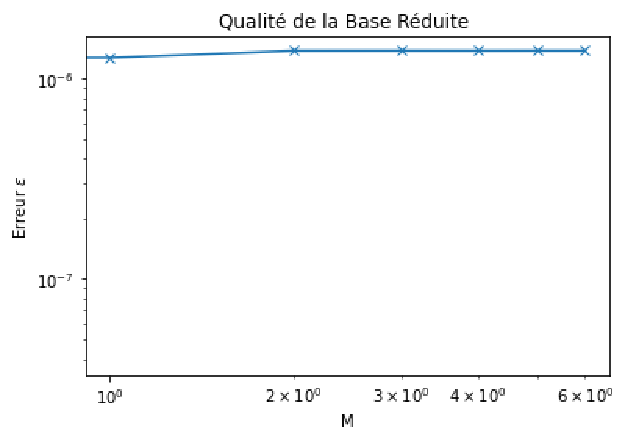
\includegraphics[scale=1]{qual_br.pdf}
\caption[]{Erreur $\epsilon$ pour différent valeur de M }
\end{center}
\label{fig:2}
\end{figure}

Maintenant on souhaite savoir sur quelles parties de $\Omega$ le modèle base réduit est le moins performant. En fixant $\mu = 0.05$ et $Nel = 100$, l'erreur absolue entre la solution éléments finis et base réduite est d'ordre $10^{-3}$ dans les intervalles $[0.4, 0.6]$, $[0.2, 0.4]$ et $[0.6, 0.8]$ d'après le graphique ci-dessous~\eqref{fig:3}.

\begin{figure}[H]
\begin{center}
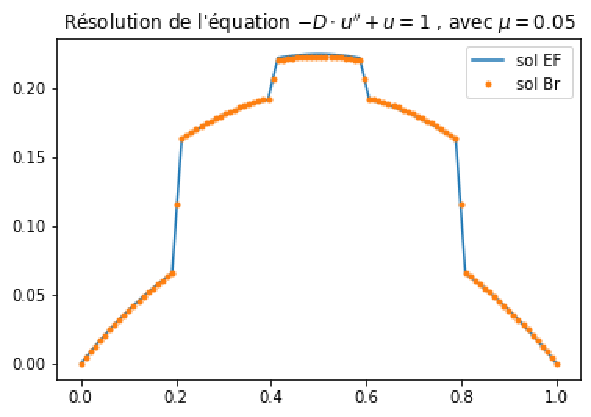
\includegraphics[scale=1]{sol_br_ef.pdf}
\caption[]{Solutions Eléments Finis et Base Réduite  }
\end{center}
\end{figure}

\begin{figure}[H]
\begin{center}
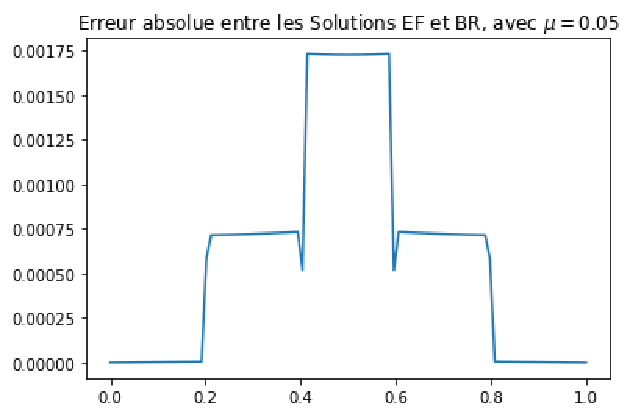
\includegraphics[scale=1]{err_br_ef.pdf}
\caption[]{Erreur  en valeur absolu entre les solutions EF et BR }
\end{center}
\label{fig:3}
\end{figure}


\section{Conclusion}

Pour conclure, nous avons résolu le cas 1D par la méthode des éléments finis et des bases réduites. Dans l'avenir, on souhaite lancer un algorithme Glouton avec le modèle par réseau de neurones à la place de l'erreur de projection pour le cas 1D et effectuer le cas 2d avec Feelpp.








\begin{thebibliography}{9}

\bibitem{Gianluigi Rozza}
Gianluigi Rozza.  \emph{An introduction to reduced basis method for parametrized PDEs, ResearchGate}

\bibitem{B. Haasdonk}
B. Haasdonk.  \emph{Reduced Basis Methods for Parametrized PDEs –
A Tutorial Introduction for Stationary and
Instationary Problems, University of Stuttgart  } 


\bibitem{Alexandre Ern}
Alexandre Ern.  \emph{ Analyse numérique et optimisation Méthode des bases réduites }\url{http://www.cmap.polytechnique.fr/~allaire/map431/MiniProjets/sujets2013/sujet9.pdf}

\bibitem{Bopeng RAO}
Bopeng RAO,  \emph{ Méthodes Numériques
des Equations aux Dérivées Partielles. UFR de Mathématique et d’Informatique
Université de Strasbourg, 2021-2022 }

\bibitem{Gwenol Grandperrin}
Gwenol Grandperrin.  \emph{Introduction à la méthode des bases réduites, ResearchGate Janvier 2008 }

\end{thebibliography}

\end{document}